\documentclass[11pt]{article}

\usepackage[left=2cm, right=2cm, top=2cm]{geometry}
\usepackage[dvipdfmx]{graphicx}
\usepackage{float}

\title{Project 1: Reaction Timer}
\author{Jacob Boline}

\begin{document}
\maketitle

\section{Introduction}
In this project I was tasked with creating and testing a design that would measure a humans response to visual stimulus. The device is required to have 3 buttons that correspond to start, stop, and clear. The basic premise of the design is to have a random delay of 2-15 seconds after the start button is pushed, but before the LED is lit. Once the LED is lit, a 4-digit display will show the number of milliseconds it takes a person to press the stop button. In addition, there are some extra features added to make the design more robust such as a state if the stop button is pushed too early, or not pushed at all. To accomplish this project Vivado 2017.2 was used to simulate, synthesize, and implement System Verilog code for a Basys 4 DDR development board.

\section{Experimental Plan}
For this design five fundamental Modules are needed:
\begin{itemize}
    \item 7-seg Driver Module
    \item Random Number Generator Module
    \item State Machine
    \item Stop Watch Module
    \item Universal Counter Module
\end{itemize}

\subsection{7-Seg Driver Module}
The first step to building this design was to create a method for driving the 7-segment display. This was accomplished by creating a decoder that had a 4-bit data in port, a 1-bit flag to indicate whether the data corresponded to numerical values, or alphabetic values, and an 8-bit data out port that corresponds to what portions of 7-segment display to turn on. Using 4 instantiations of this decoder, and the display mux from listing 4.15 in the class textbook I created a driver module (as seen in Figure \ref{fig:7SegDriver}) that had 4 separately controlled digits, and could display the numbers 0-9 and the letters H and I.

\begin{figure}[H]
	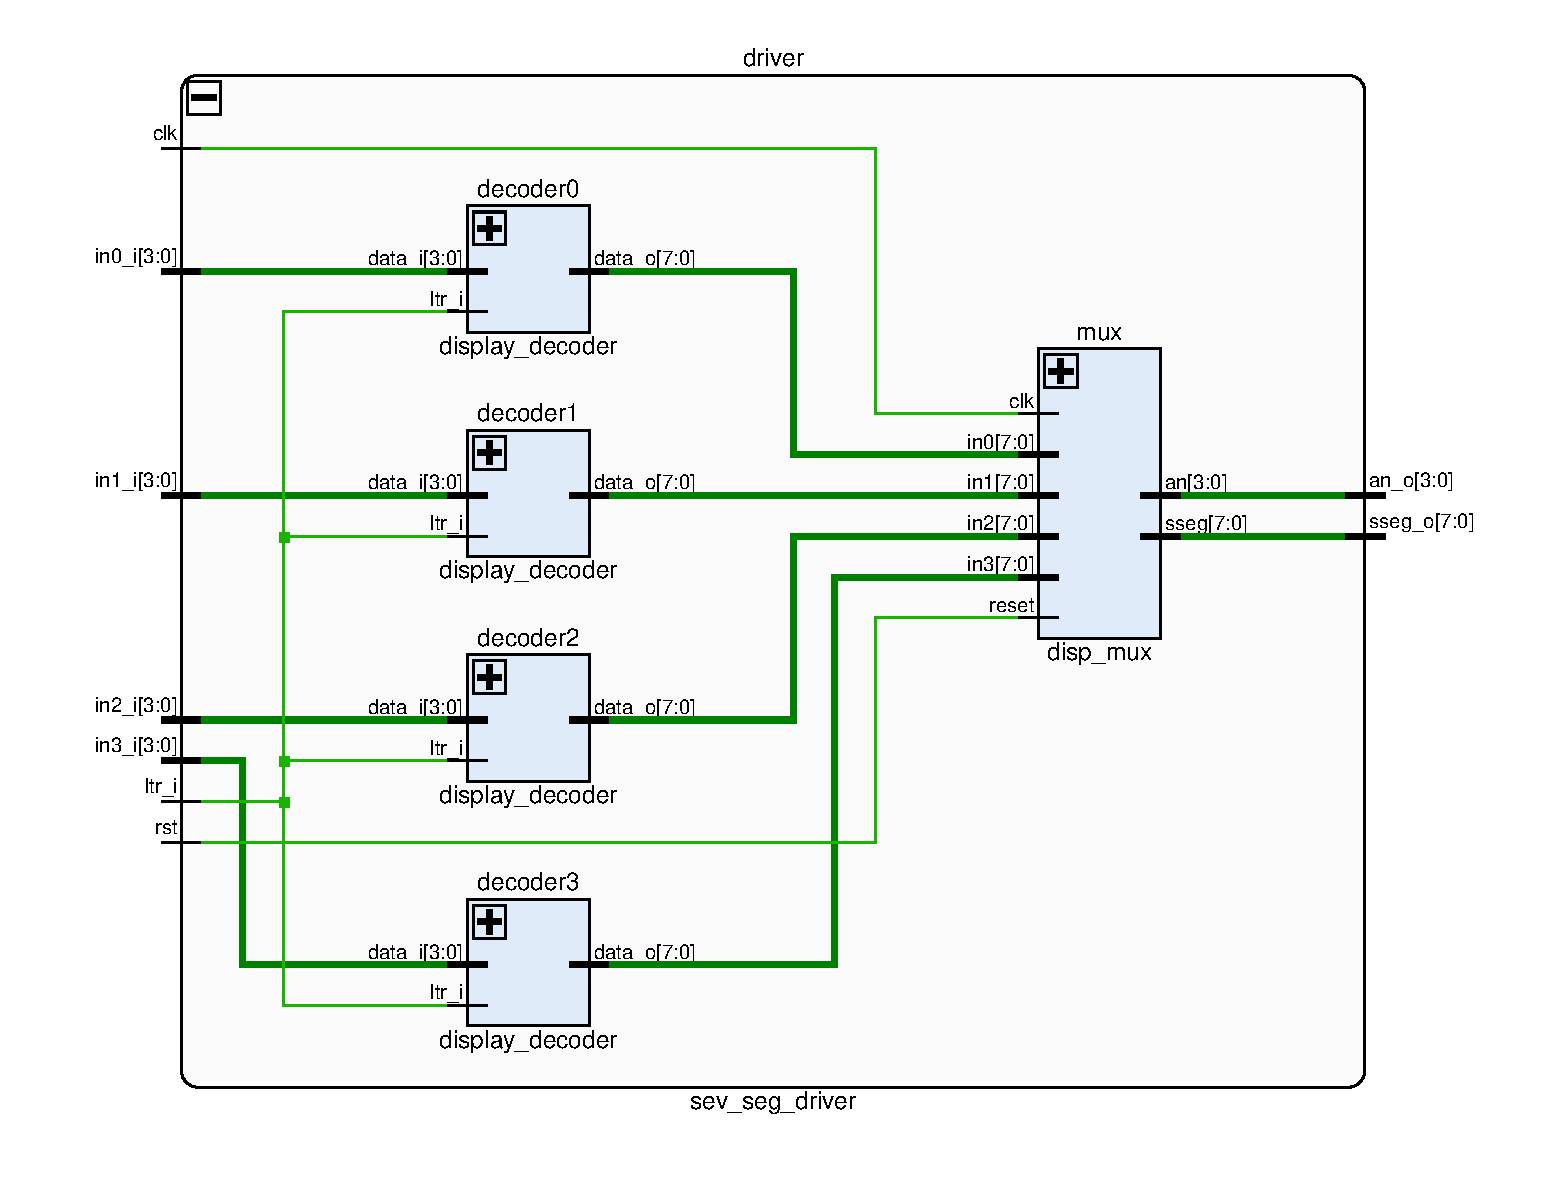
\includegraphics [width=5in]{display_driver.eps}
	\centering
	\caption{Block diagram of 7-seg driver module.}
	\label{fig:7SegDriver}
\end{figure}


\subsection{Random Number Generator Module}


\pagebreak
\begin{figure}[H]
	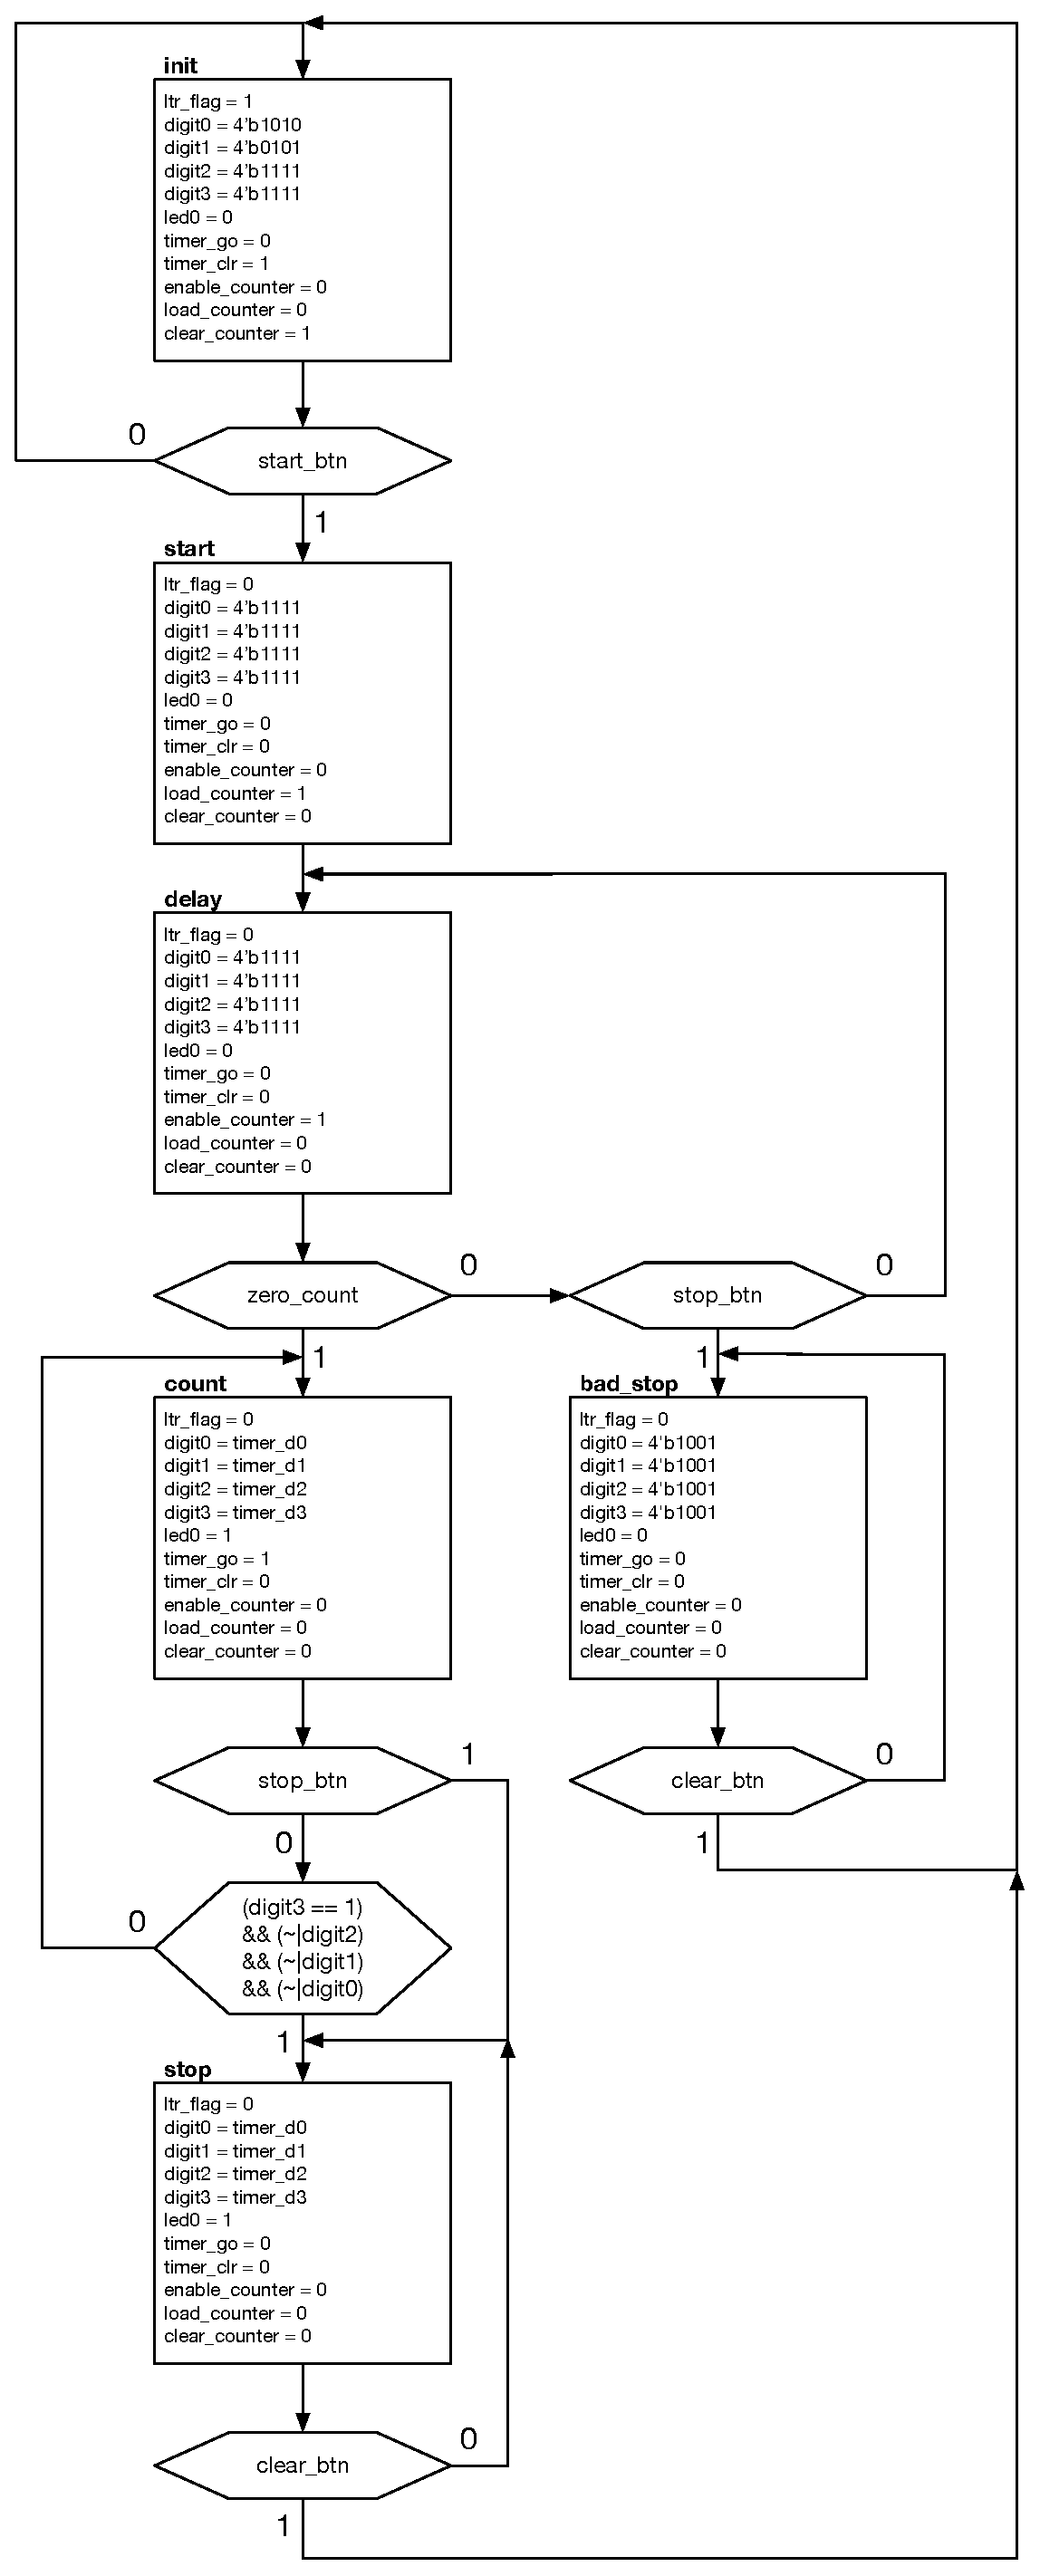
\includegraphics [width=3.45in]{state_diagram.eps}
	\centering
	\caption{State diagram of the reaction timer design}
	\label{fig:state_diagram}
\end{figure}

\section{Analysis}

\section{Conclusion}

\end{document}